\documentclass[]{article}
\usepackage{lmodern}
\usepackage{amssymb,amsmath}
\usepackage{ifxetex,ifluatex}
\usepackage{fixltx2e} % provides \textsubscript
\ifnum 0\ifxetex 1\fi\ifluatex 1\fi=0 % if pdftex
  \usepackage[T1]{fontenc}
  \usepackage[utf8]{inputenc}
\else % if luatex or xelatex
  \ifxetex
    \usepackage{mathspec}
  \else
    \usepackage{fontspec}
  \fi
  \defaultfontfeatures{Ligatures=TeX,Scale=MatchLowercase}
\fi
% use upquote if available, for straight quotes in verbatim environments
\IfFileExists{upquote.sty}{\usepackage{upquote}}{}
% use microtype if available
\IfFileExists{microtype.sty}{%
\usepackage[]{microtype}
\UseMicrotypeSet[protrusion]{basicmath} % disable protrusion for tt fonts
}{}
\PassOptionsToPackage{hyphens}{url} % url is loaded by hyperref
\usepackage[unicode=true]{hyperref}
\hypersetup{
            pdftitle={Recovering theta from volume scaling exponents},
            pdfborder={0 0 0},
            breaklinks=true}
\urlstyle{same}  % don't use monospace font for urls
\usepackage[margin=1in]{geometry}
\usepackage{graphicx,grffile}
\makeatletter
\def\maxwidth{\ifdim\Gin@nat@width>\linewidth\linewidth\else\Gin@nat@width\fi}
\def\maxheight{\ifdim\Gin@nat@height>\textheight\textheight\else\Gin@nat@height\fi}
\makeatother
% Scale images if necessary, so that they will not overflow the page
% margins by default, and it is still possible to overwrite the defaults
% using explicit options in \includegraphics[width, height, ...]{}
\setkeys{Gin}{width=\maxwidth,height=\maxheight,keepaspectratio}
\IfFileExists{parskip.sty}{%
\usepackage{parskip}
}{% else
\setlength{\parindent}{0pt}
\setlength{\parskip}{6pt plus 2pt minus 1pt}
}
\setlength{\emergencystretch}{3em}  % prevent overfull lines
\providecommand{\tightlist}{%
  \setlength{\itemsep}{0pt}\setlength{\parskip}{0pt}}
\setcounter{secnumdepth}{0}
% Redefines (sub)paragraphs to behave more like sections
\ifx\paragraph\undefined\else
\let\oldparagraph\paragraph
\renewcommand{\paragraph}[1]{\oldparagraph{#1}\mbox{}}
\fi
\ifx\subparagraph\undefined\else
\let\oldsubparagraph\subparagraph
\renewcommand{\subparagraph}[1]{\oldsubparagraph{#1}\mbox{}}
\fi

% set default figure placement to htbp
\makeatletter
\def\fps@figure{htbp}
\makeatother


\title{Recovering theta from volume scaling exponents}
\author{}
\date{\vspace{-2.5em}}

\begin{document}
\maketitle

Using the volume scaling methodology for calculating empirical metabolic
scaling exponents, we can compare our newer, more accurate results to
those derived from the predictions of WBE theory using branching traits:

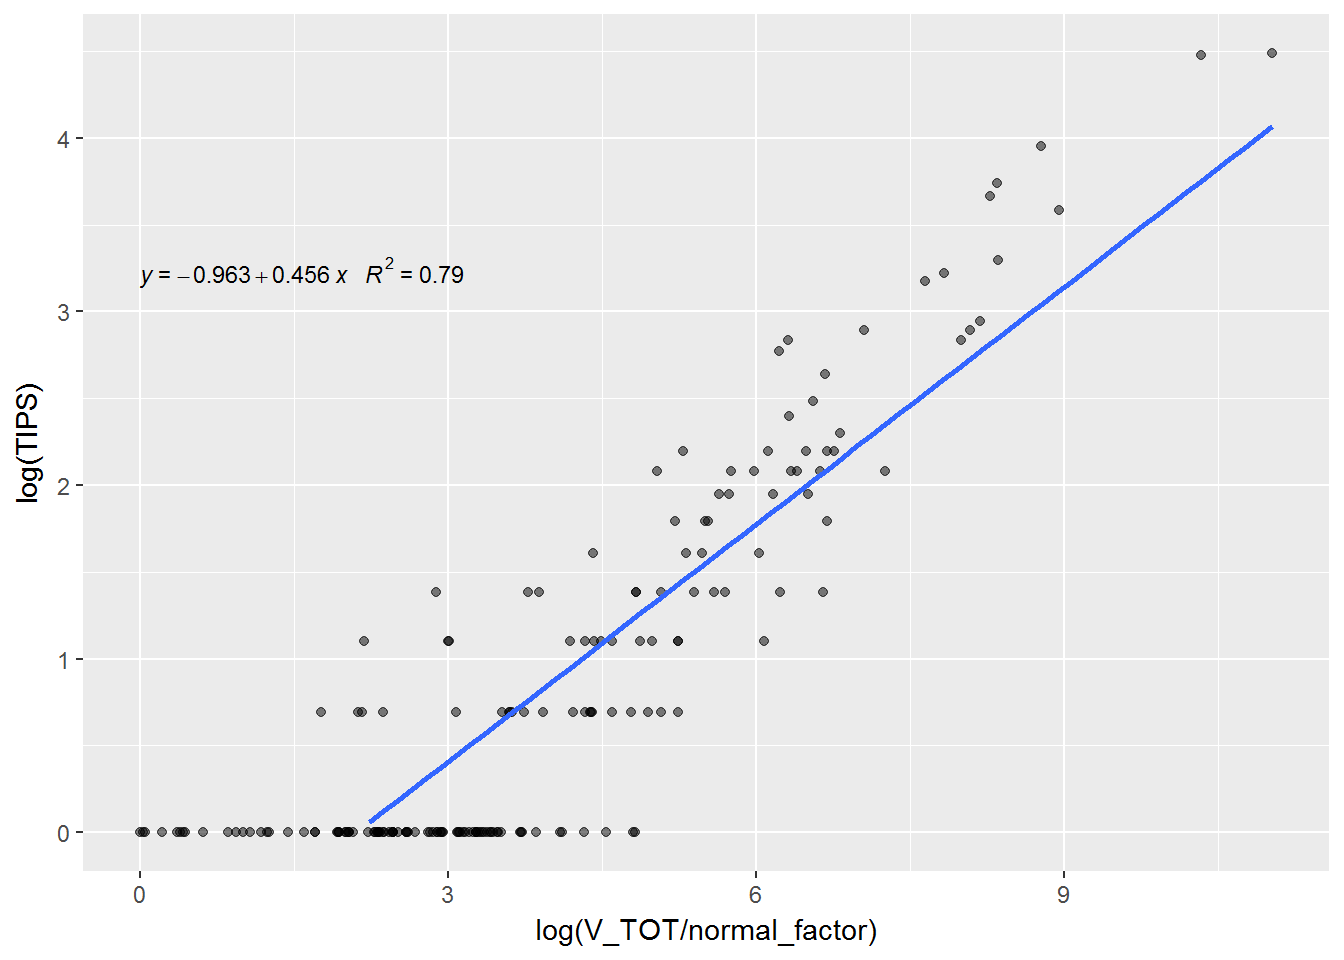
\includegraphics{recovering_theta_files/figure-latex/unnamed-chunk-1-1.pdf}

With a slope of 0.48, our calculated exponents weakly predict the
empirical exponents coming out of the volume scaling approach. This at
least shows some consistency between theoretical and empirical
approaches, and may indicate that our theta values are merely
systematically biased downward rather than entirely incorrect.

We are left to explore the distribution of volume scaling slopes for
answers about the true theta values for these trees. A basic and
encouraging result is that volume scaling is independent of the total
size of the tree:

\includegraphics{recovering_theta_files/figure-latex/unnamed-chunk-2-1.pdf}

By genus:

\includegraphics{recovering_theta_files/figure-latex/unnamed-chunk-3-1.pdf}

Variation in volume scaling exponents could reflect real life-history
variation, which would correlate with other traits along a fast-slow
continuum. In this case, lower exponents (closer to 0) represent a
slow-growing strategy, while exponents closer to 1 would reflect a
fast-growing strategy. We attempt to test for this relationship below
using traits from the BIEN database. First, our life history traits will
be represented by wood density and SLA, which should exhibit a negative
correlation along the fast-slow continuum. Unfortunately, we are not
able to recover this relationship from the species present in our
dataset:

\includegraphics{recovering_theta_files/figure-latex/unnamed-chunk-4-1.pdf}

Correspondingly, the relationships with our volume scaling exponent are
quite weak.

\includegraphics{recovering_theta_files/figure-latex/unnamed-chunk-5-1.pdf}

\includegraphics{recovering_theta_files/figure-latex/unnamed-chunk-6-1.pdf}

Encouragingly, the relationship with SLA is in the right direction, .

\end{document}
